\documentclass{article}
\usepackage{ctex}
\usepackage{graphicx}
\usepackage{amsmath}
\usepackage{indentfirst}
\usepackage{titlesec}
\usepackage{setspace}
\usepackage{subfigure}
\usepackage{caption}
\usepackage{float}
\usepackage{booktabs}
\usepackage{geometry}
\usepackage{multirow}
\usepackage{hyperref}
\hypersetup{
	colorlinks=true,
	linkcolor=blue,
	filecolor=magenta,      
	urlcolor=cyan,
	pdftitle={Overleaf Example},
	pdfpagemode=FullScreen,
}
\geometry{left=1.2cm,right=1.2cm,top=2cm,bottom=2cm}
\title{\songti \zihao{2}\bfseries HW9第15题Markov链2维模拟}
\titleformat*{\section}{\songti\zihao{4}\bfseries}
\titleformat*{\subsection}{\songti\zihao{5}\bfseries}
\renewcommand\thesection{\arabic{section}}
\author{王启骅 PB20020580}
\begin{document}
	\maketitle
	\section{题目}
	设体系的能量为$ H(x,y)=-2(x^2+y^2)+\frac{1}{2}(x^4+y^4)+\frac{1}{2}(x-y)^4 $ ,取$\beta=0.2,\ 1,1 5$ ,
	采用Metropolis抽样法计算$ \langle x^2\rangle,\ \langle y^2\rangle,\ \langle x^2+y^2\rangle $ 。抽样时在2维平面上依次标出Markov链点
	分布,从而形象地理解Markov链。
	\section{算法原理}
	对于正则系统,有分布
	\begin{equation}
		p(x,y)=\frac{1}{Z}\exp[-\beta H(x,y)]
	\end{equation}
其中配分函数
\begin{equation}
	Z=\int_{-\infty}^{+\infty}\int_{-\infty}^{+\infty}\exp(-\beta H)dxdy
\end{equation}


对于求解平均值
\begin{equation}
	\langle x^2\rangle=\int_{-\infty}^{+\infty}\int_{-\infty}^{+\infty}x^2\ p(x,y)\ dxdy
\end{equation}
\begin{equation}
	\langle y^2\rangle=\int_{-\infty}^{+\infty}\int_{-\infty}^{+\infty}y^2\ p(x,y)\ dxdy
\end{equation}
\begin{equation}
	\langle x^2+y^2\rangle=\int_{-\infty}^{+\infty}\int_{-\infty}^{+\infty}(x^2+y^2)\ p(x,y)\ dxdy
\end{equation}


进行metropolis方法抽样模拟Markov链,首先选取初始坐标$ (x_0,y_0) $,从此开始游走。抽取[0,1]均匀分布的随机数$ \xi $,则每次随机行走的位移$ \delta=(\xi-0.5)\Delta $,接受该移动的几率为
\begin{equation}
	p_{\alpha}=\min\{1,\exp[-\beta(H_1-H_0)]\}
\end{equation}
领取一个新的随机数$ \xi>p_{\alpha} $时,拒受该构型,保持原构型不变,否则接受。每次记录新随机游走点的坐标,进行平均值求解。
\begin{equation}
	\langle A\rangle=\frac{1}{n-m}\sum_{m+1}^{n}A
\end{equation}
其中前m为热化过程舍去。
	\section{结果}
	这里取用n=$ 10^6 $个点进行模拟,取前$ m=10^5 $作为热化过程。并取每次位移距离$ \Delta=2 $。
	\subsection{$\beta=0.2$}
	计算得到结果
	\begin{equation}
		\langle x^2\rangle=1.5732543080442860
	\end{equation}
\begin{equation}
	\langle x^2\rangle=1.5621809210996516
\end{equation}
\begin{equation}
	\langle x^2+y^2\rangle=3.1354352291439378
\end{equation}
对比计算得到标准结果为
	\begin{equation}
	\langle x^2\rangle_{standard}=\langle y^2\rangle_{standard}=1.561886003600077
\end{equation}
\begin{equation}
	\langle x^2+ y^2\rangle_{standard}=3.123771904782158
\end{equation}
二维Markov链如图\ref{fig:1}
	\begin{figure}[!h]
	
	\centering
	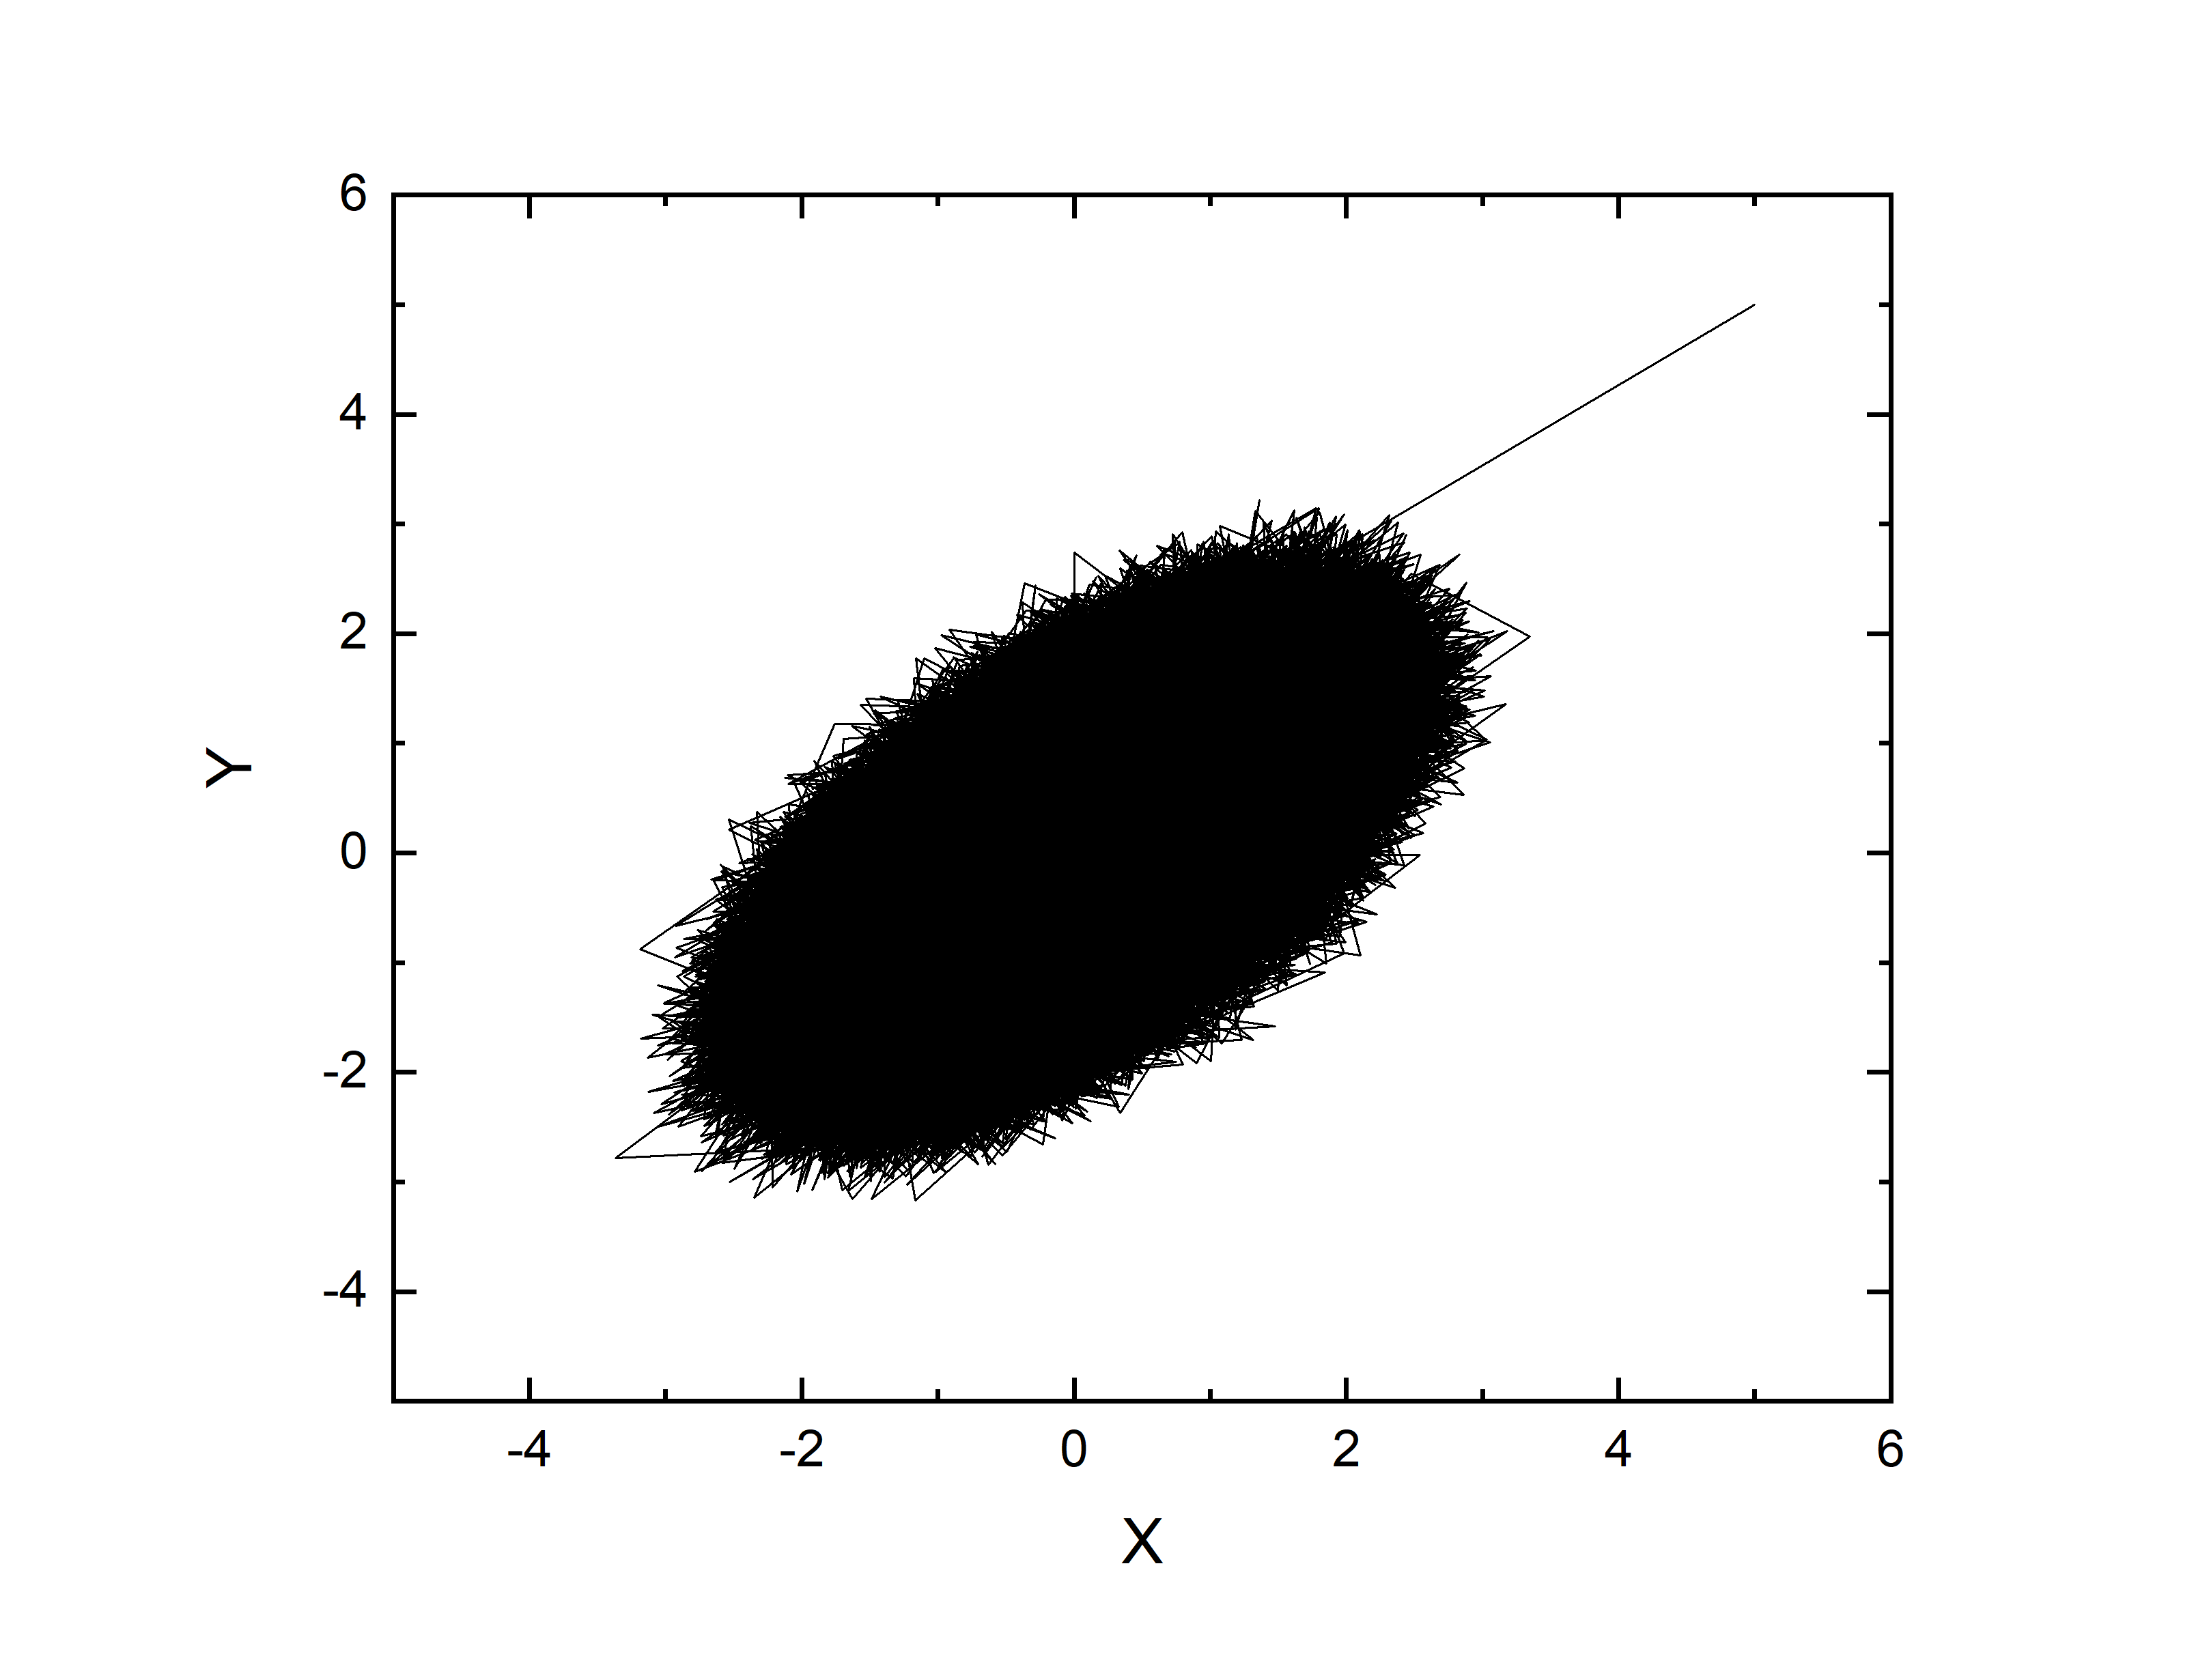
\includegraphics[scale=0.6]{beta02}
	\captionsetup{font={small},labelfont=bf}
	\caption{\heiti\zihao{-5}$ \beta=0.2 $下Markov链}
	\label{fig:1}
\end{figure}

	\subsection{$\beta=1$}
计算得到结果
\begin{equation}
	\langle x^2\rangle=1.6802036533334823
\end{equation}
\begin{equation}
	\langle x^2\rangle=1.6872743155871015
\end{equation}
\begin{equation}
	\langle x^2+y^2\rangle=3.3674779689205838 
\end{equation}
对比计算得到标准结果为
\begin{equation}
	\langle x^2\rangle_{standard}=\langle y^2\rangle_{standard}=1.682470341271205
\end{equation}
\begin{equation}
	\langle x^2+ y^2\rangle_{standard}=3.364940624409566
\end{equation}
二维Markov链如图\ref{fig:2}
\begin{figure}[!h]
	
	\centering
	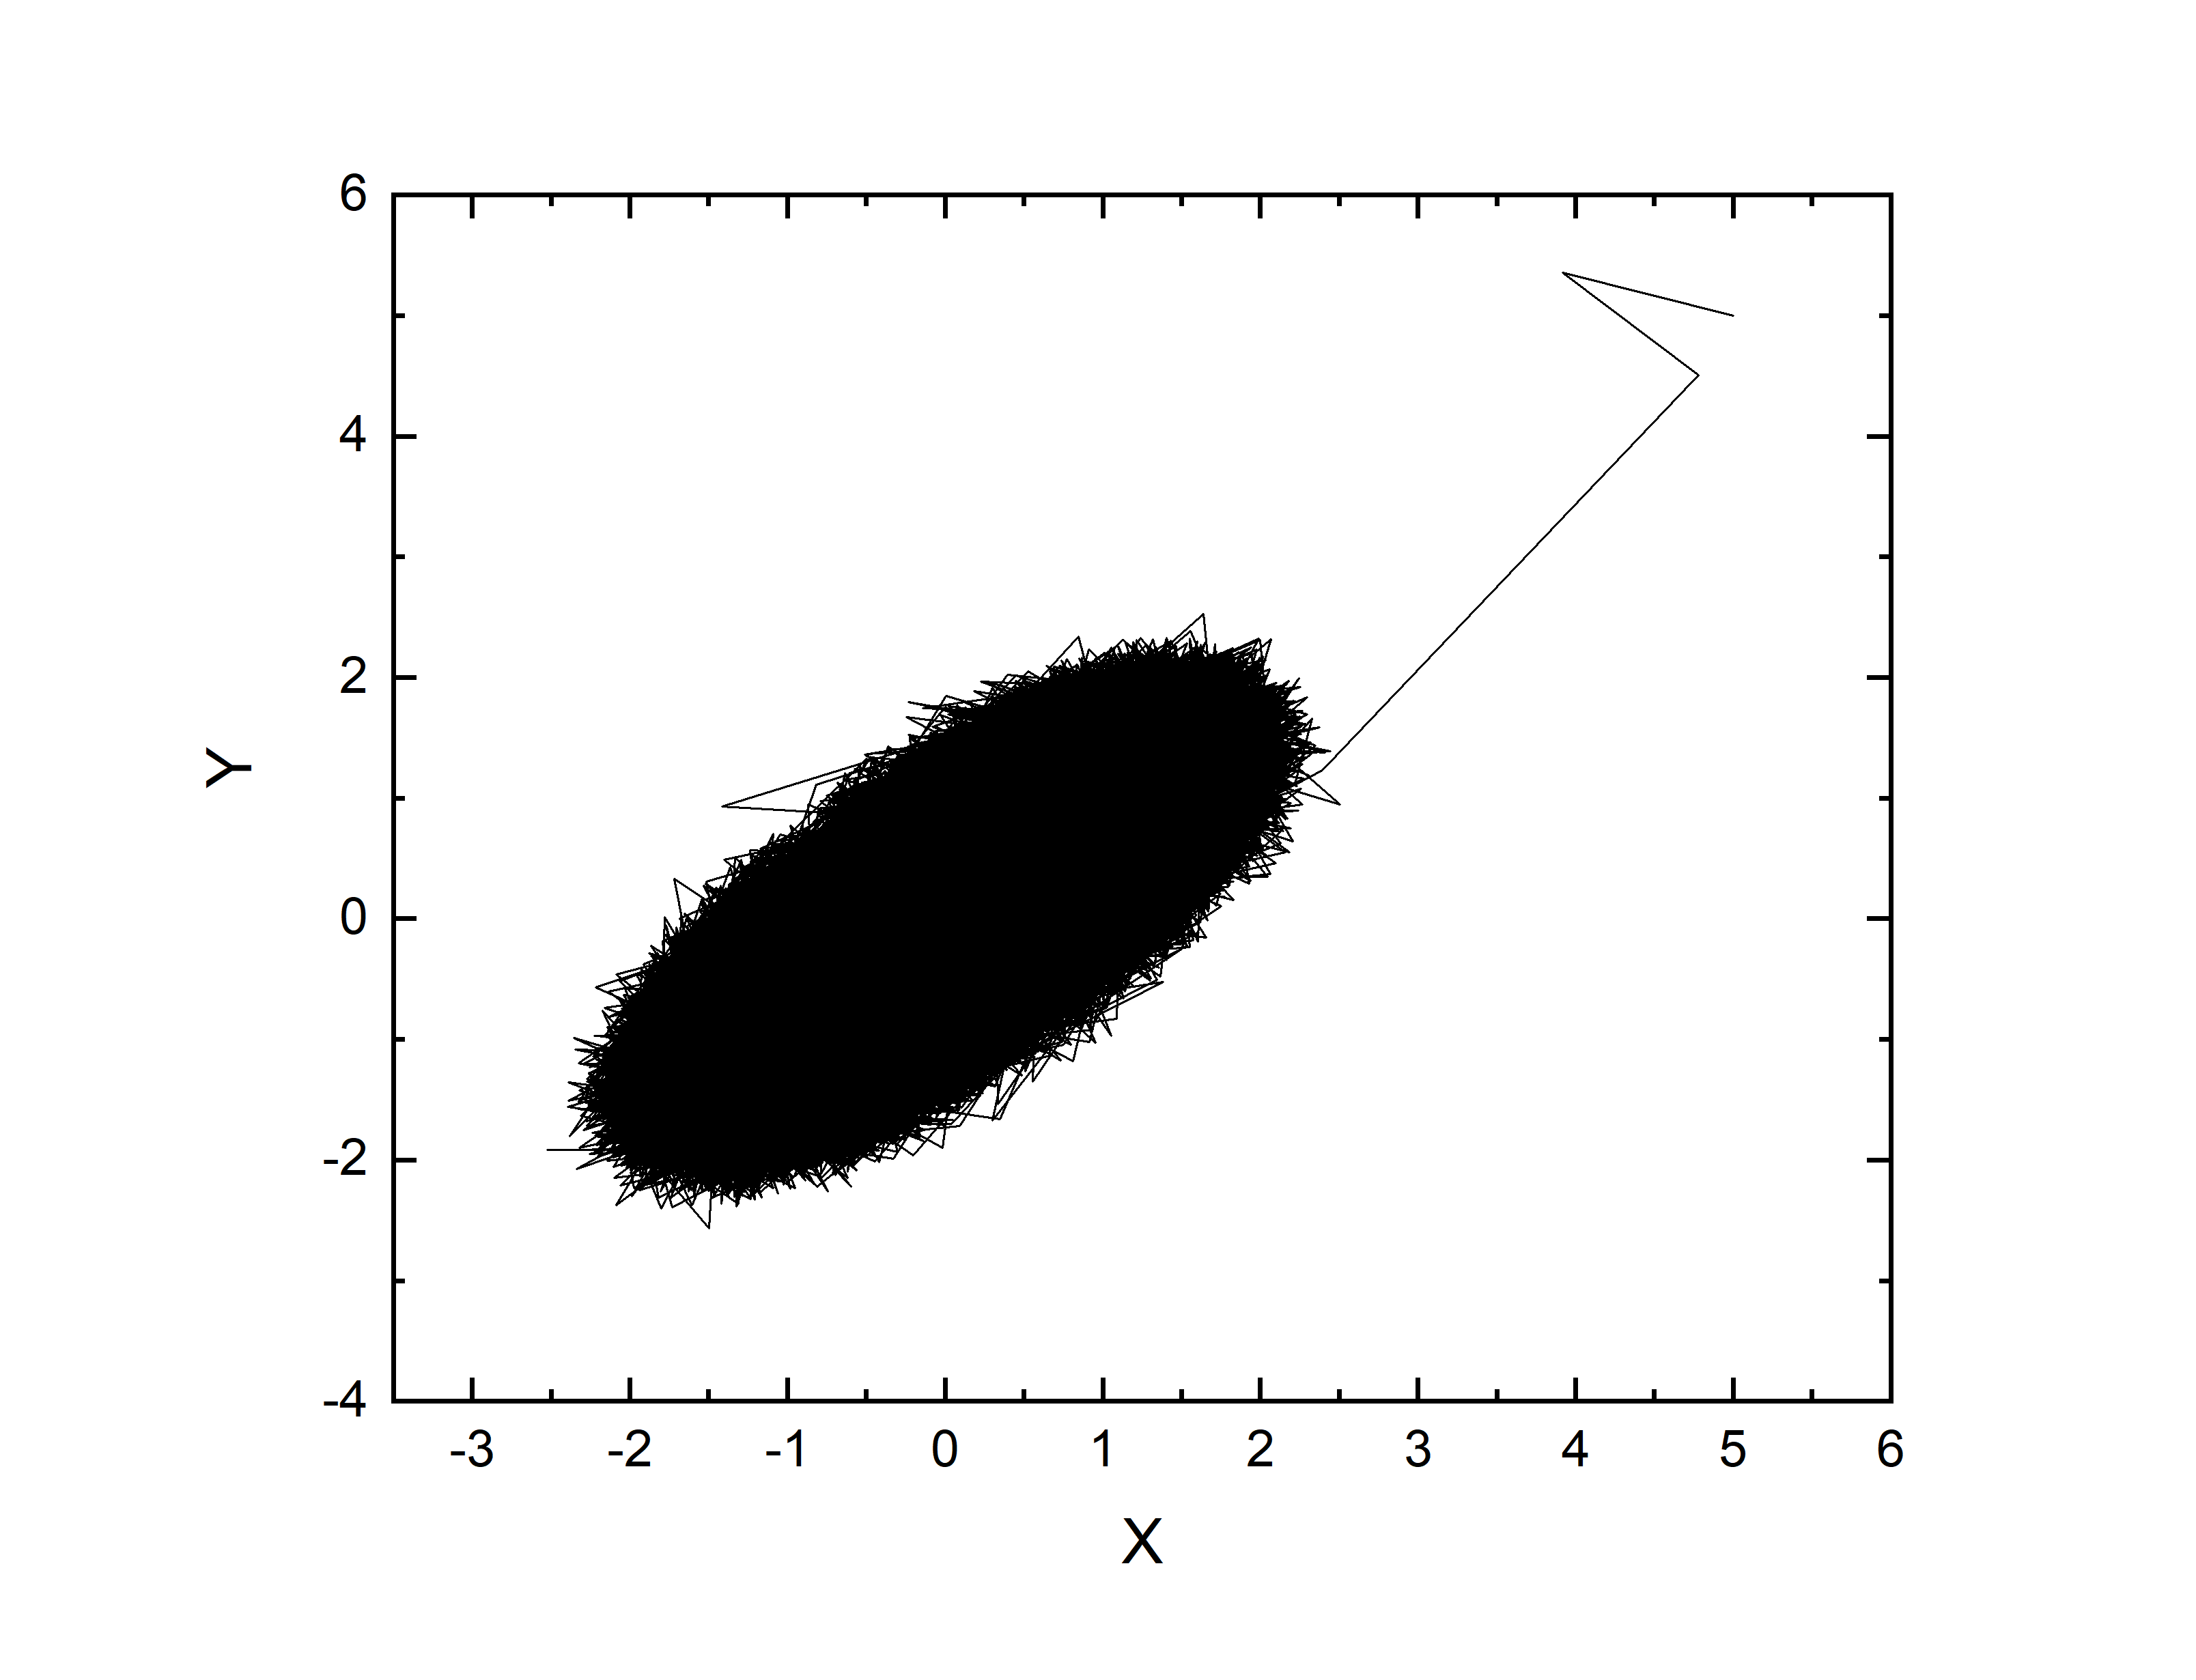
\includegraphics[scale=0.6]{beta1}
	\captionsetup{font={small},labelfont=bf}
	\caption{\heiti\zihao{-5}$ \beta=1 $下Markov链}
	\label{fig:2}
\end{figure}

	\subsection{$\beta=5$}
计算得到结果
\begin{equation}
	\langle x^2\rangle=1.9495791449383584
\end{equation}
\begin{equation}
	\langle x^2\rangle=1.9467188325009992
\end{equation}
\begin{equation}
	\langle x^2+y^2\rangle=3.8962979774393576 
\end{equation}
对比计算得到标准结果为
\begin{equation}
	\langle x^2\rangle_{standard}=\langle y^2\rangle_{standard}=1.947830003176043
\end{equation}
\begin{equation}
	\langle x^2+ y^2\rangle_{standard}=3.895659879435674
\end{equation}
二维Markov链如图\ref{fig:3}
\begin{figure}[!h]
	
	\centering
	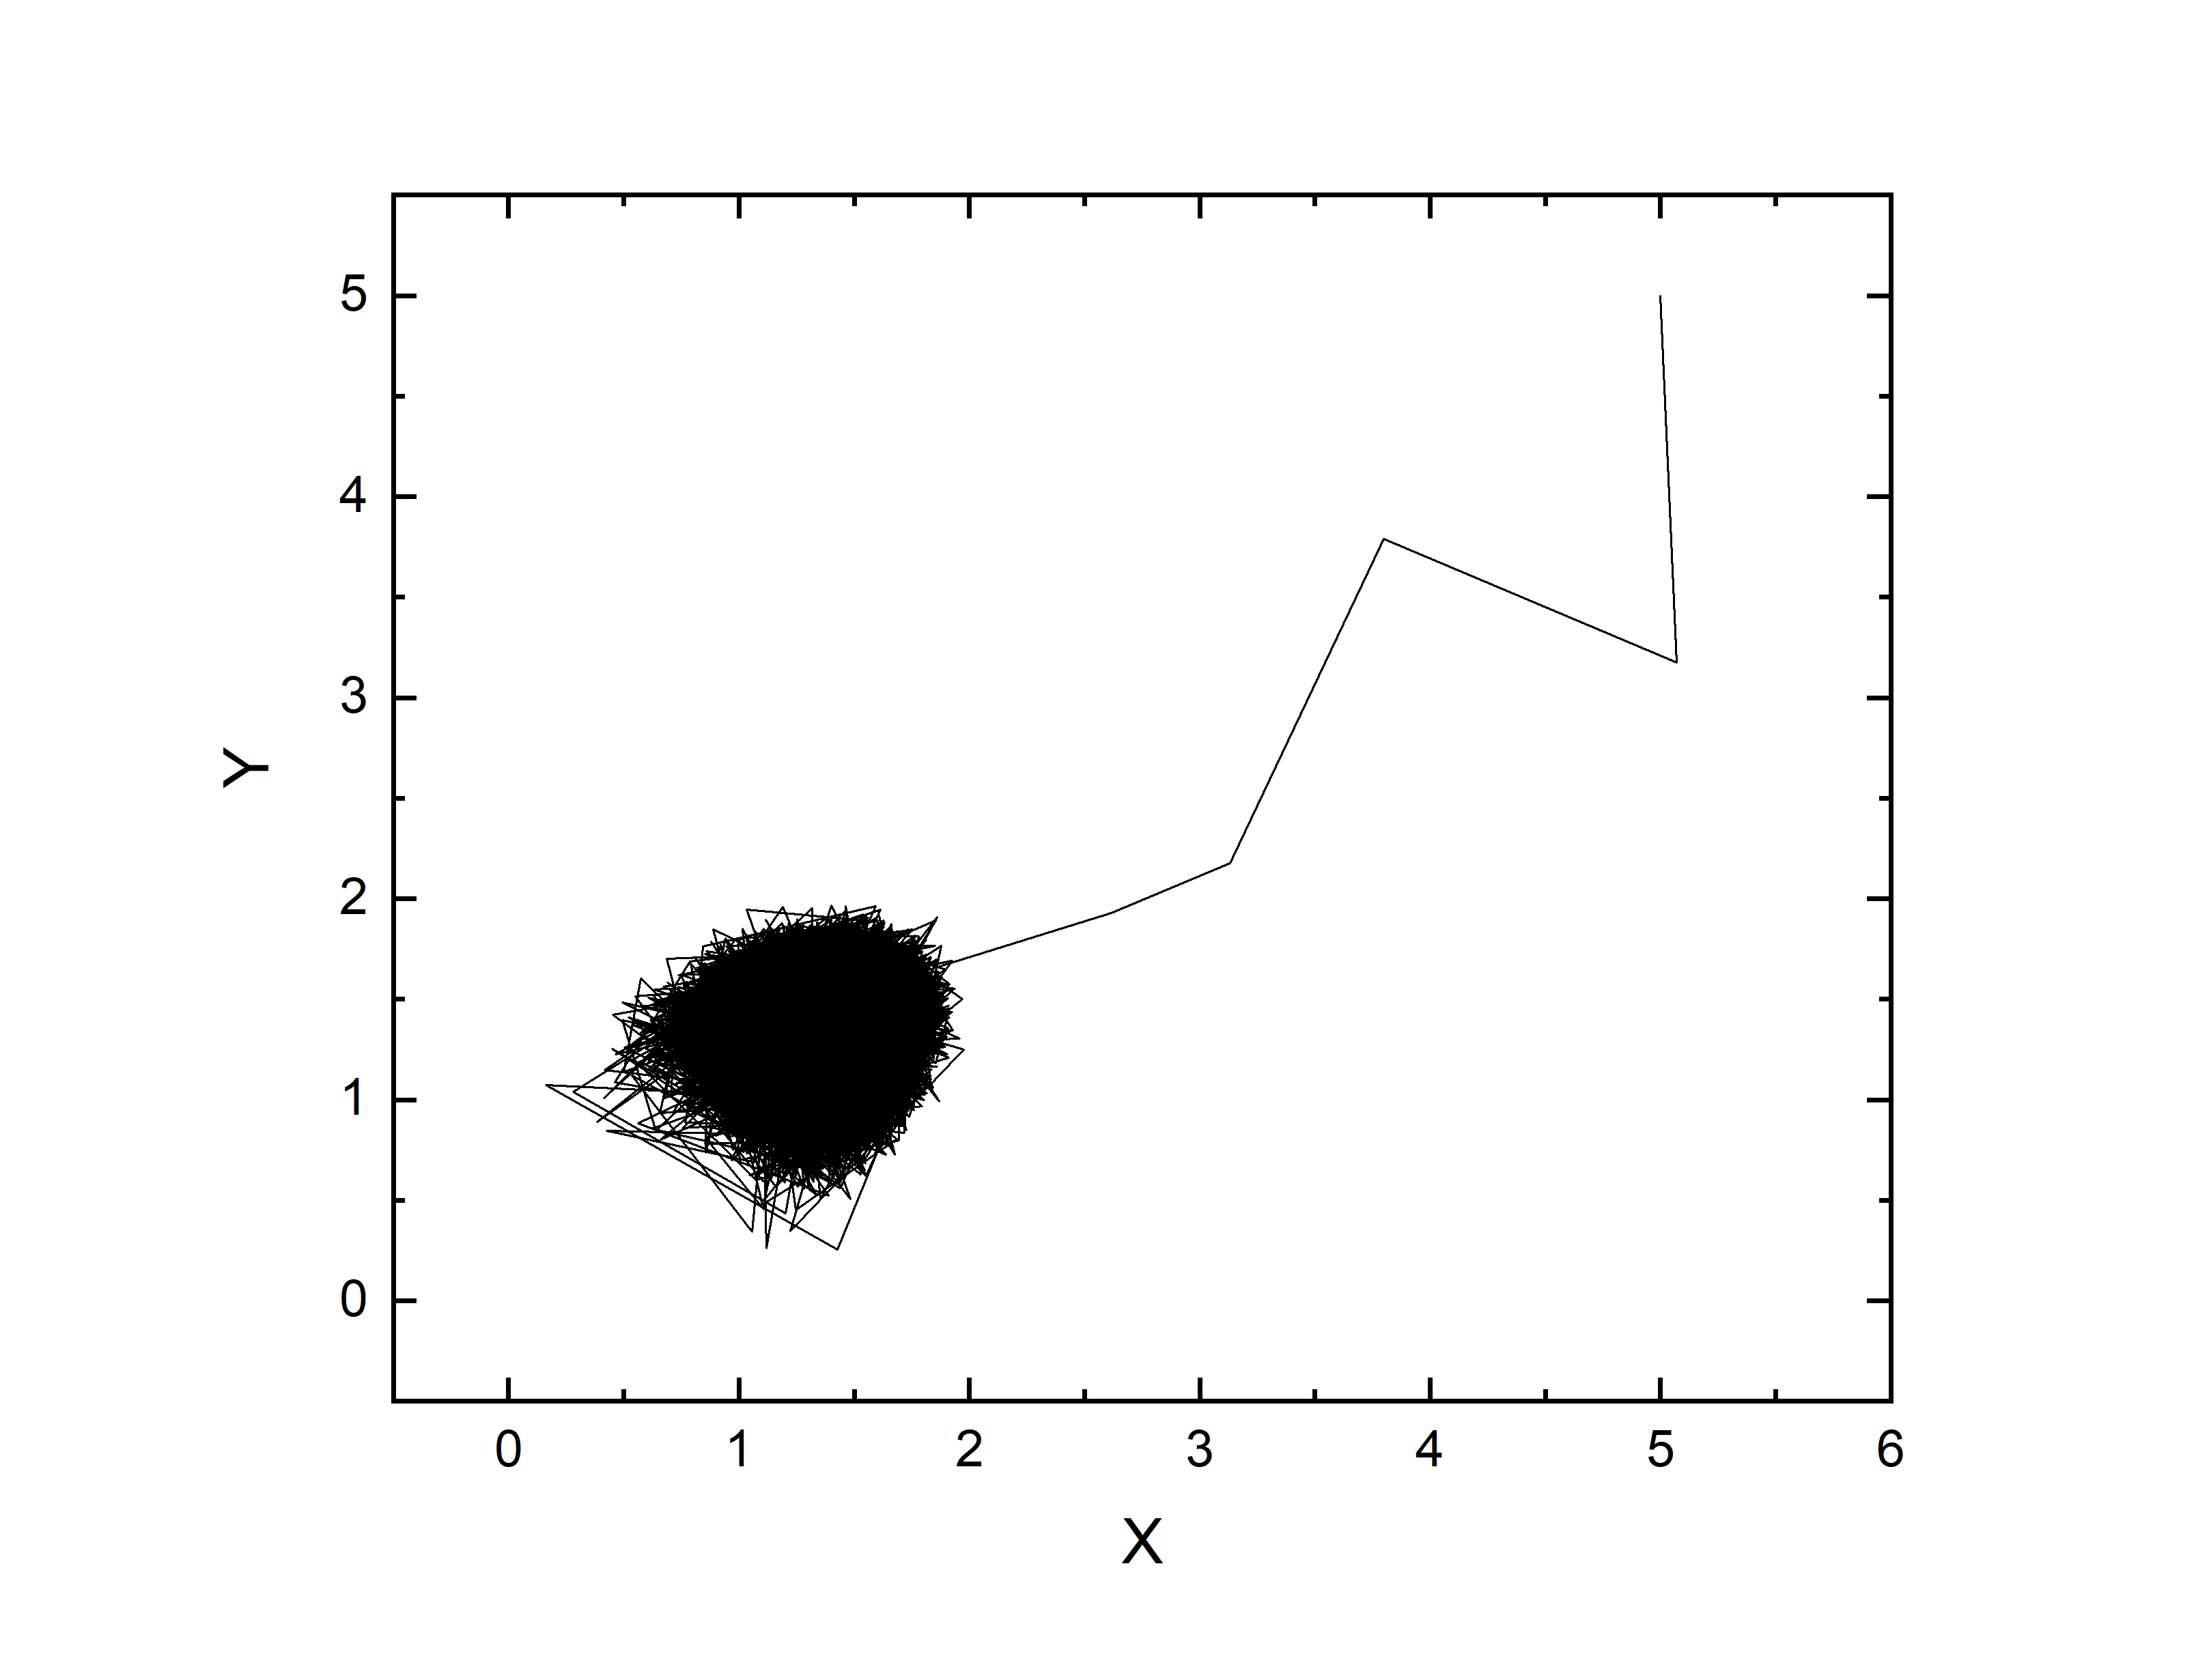
\includegraphics[scale=0.6]{beta5}
	\captionsetup{font={small},labelfont=bf}
	\caption{\heiti\zihao{-5}$ \beta=5 $下Markov链}
	\label{fig:3}
\end{figure}	
	\subsection{误差分析}
	这里计算的平均值于标准期望值对比,具有2-3位有效数字的精度,考虑到程序运行时间问题只取了$  n=10^6 $个点,如果进一步增大取点数量级,可以达到更高精确度。
	
	
	接下来进行通过改变模拟的步数得到计算结果于真实值的绝对误差。模拟计算值的绝对误差为$ |\langle A\rangle-\langle A\rangle_{standard}| $。
	
	
		取$ \beta=0.2 $情况下。得到结果如图\ref{fig:4}
	\begin{figure}[!h]
		
		\centering
		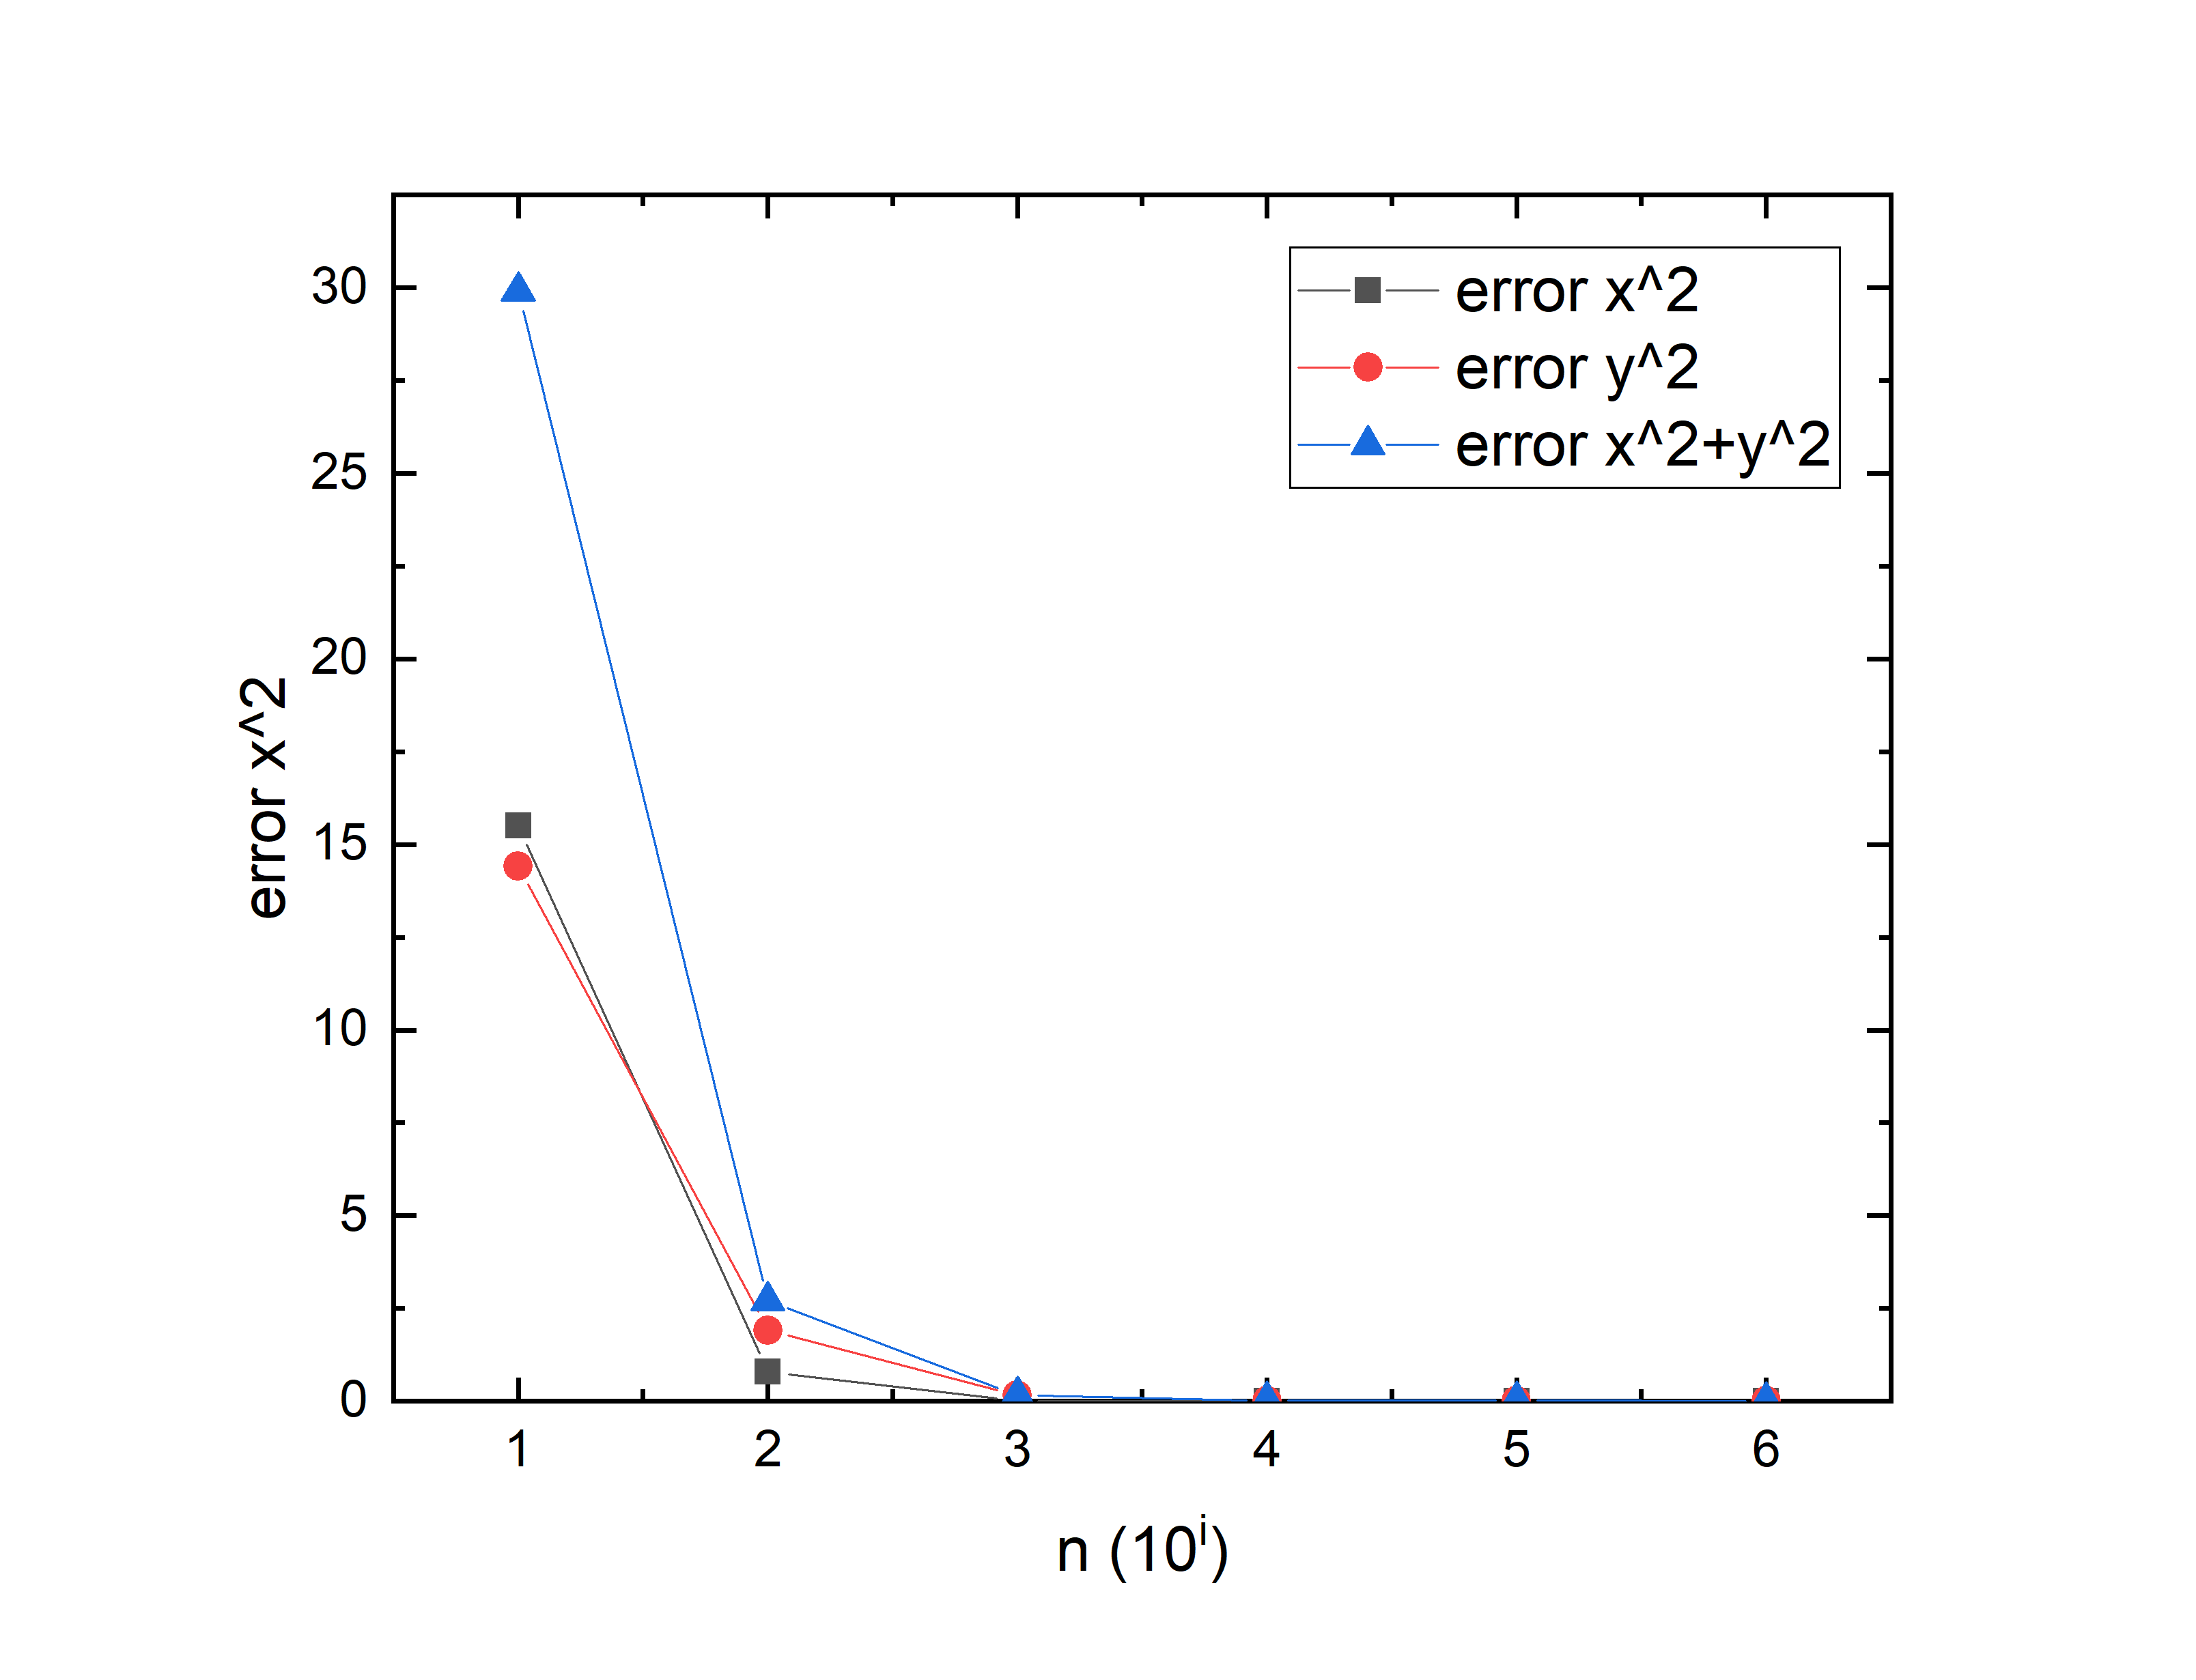
\includegraphics[scale=0.5]{error02}
		\captionsetup{font={small},labelfont=bf}
		\caption{\heiti\zihao{-5}$ \beta=0.2 $下平均值绝对误差随模拟步数变化}
		\label{fig:4}
	\end{figure}
	
		取$ \beta=1 $情况下。得到结果如图\ref{fig:5}
	\begin{figure}[!h]
		
		\centering
		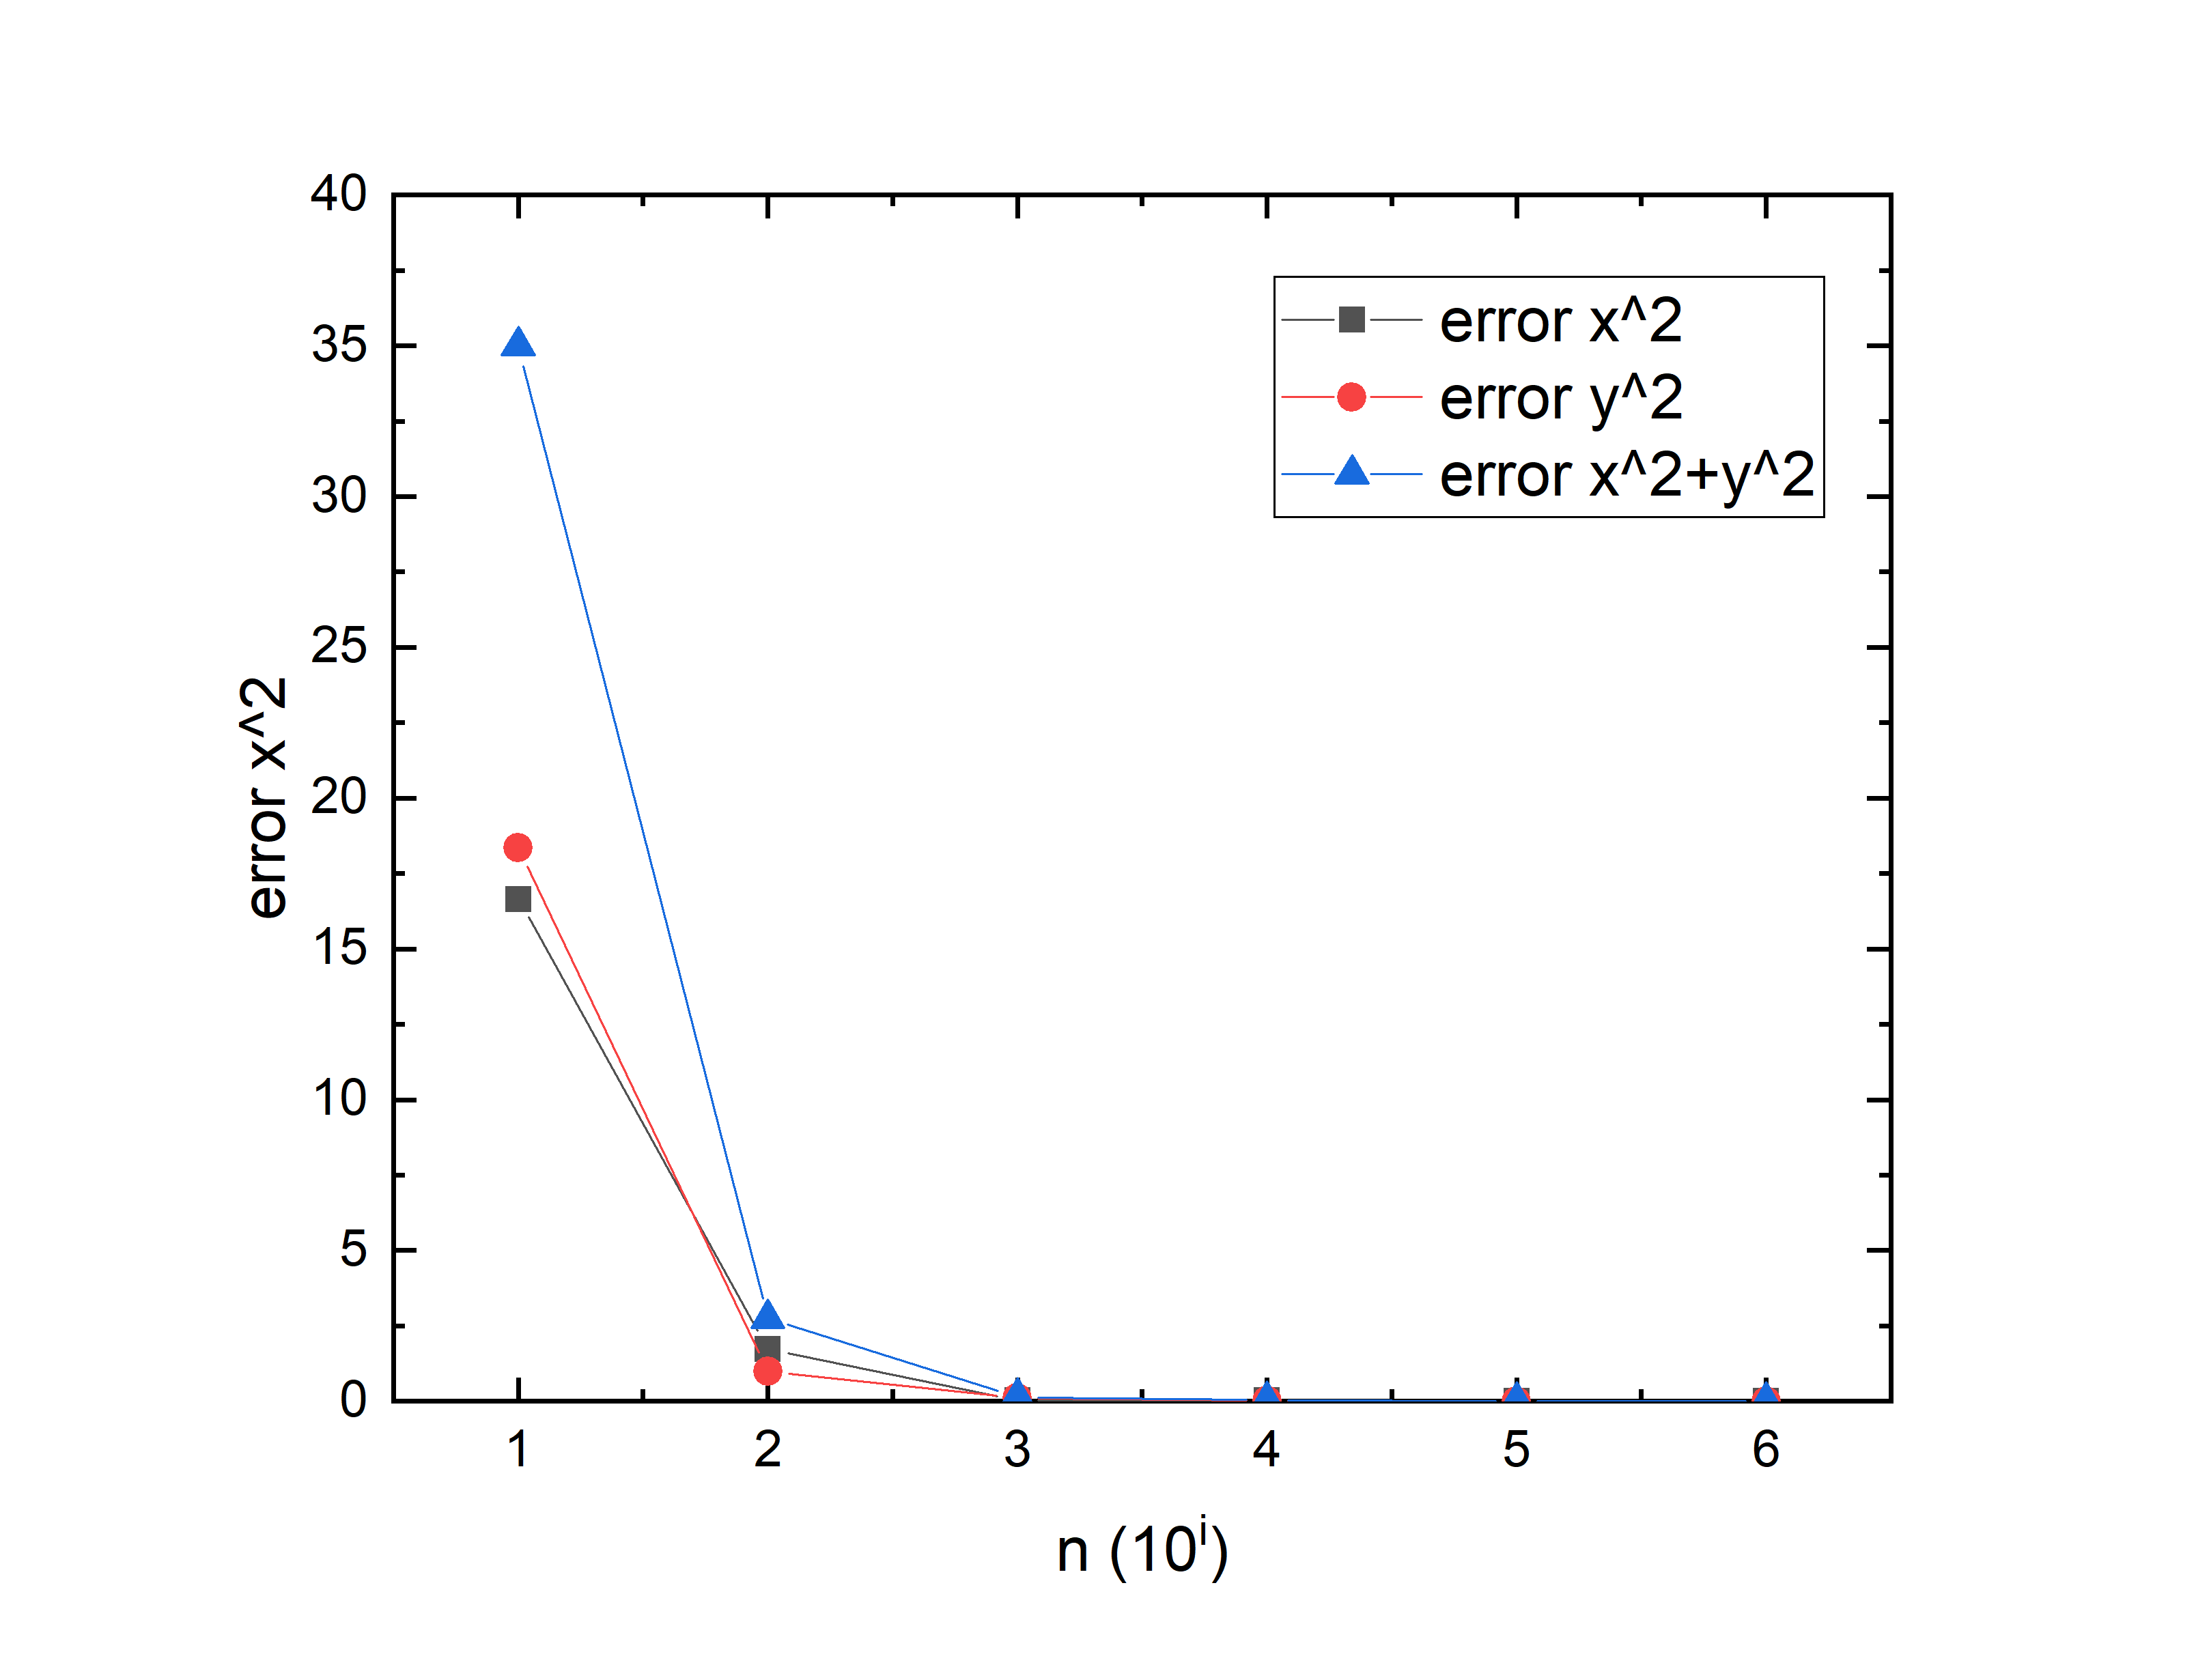
\includegraphics[scale=0.5]{error1}
		\captionsetup{font={small},labelfont=bf}
		\caption{\heiti\zihao{-5}$ \beta=1 $下平均值绝对误差随模拟步数变化}
		\label{fig:5}
	\end{figure}
	取$ \beta=5 $情况下。得到结果如图\ref{fig:6}
	\begin{figure}[!h]
		
		\centering
		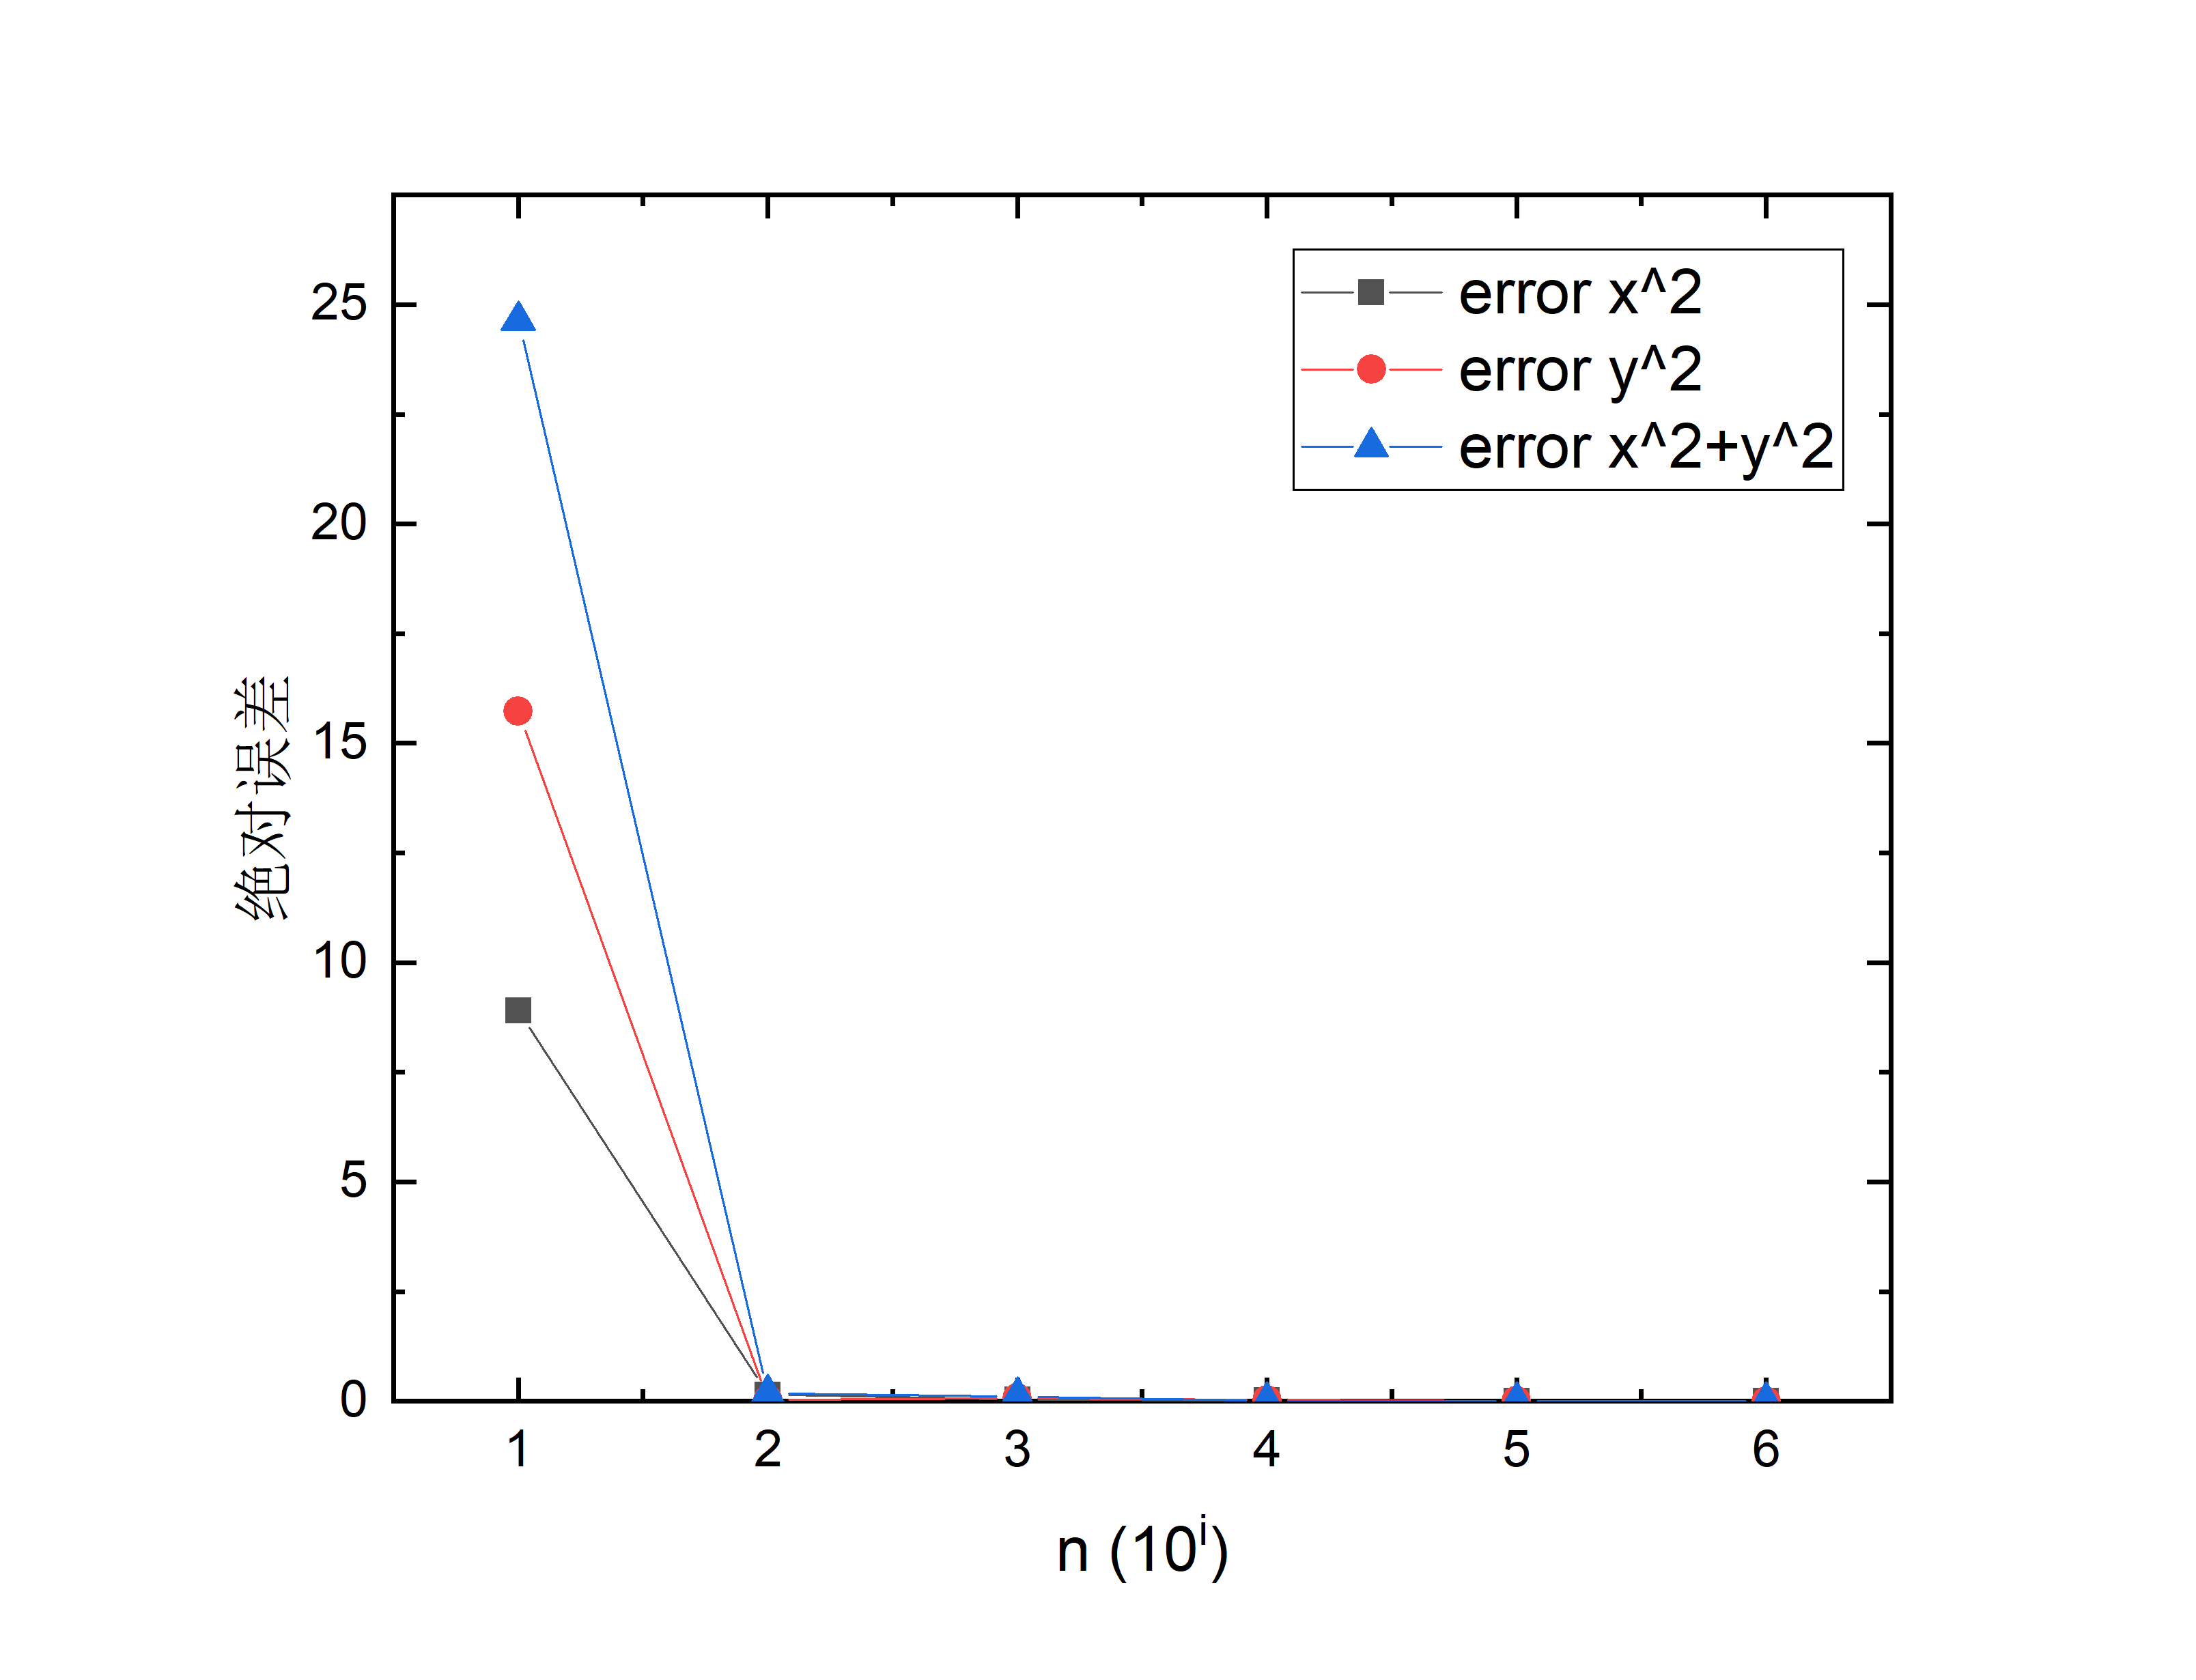
\includegraphics[scale=0.5]{error}
		\captionsetup{font={small},labelfont=bf}
		\caption{\heiti\zihao{-5}$ \beta=5 $下平均值绝对误差随模拟步数变化}
		\label{fig:6}
	\end{figure}
由图可见,在$ n=10-10^3 $误差迅速下降,从当n>$ 10^4 $后绝对误差趋近于0,基本没有太大变化。
	\section{结论}
	根据模拟结果与误差分析结果可以看出,随着$ \beta $逐渐增大,明显Markov链收敛于能量最低点的速率加快,而且在最低点附近游走的范围较小。这是由于$ \beta $增大导致游走到新的能量更高的点的概率明显减小,导致每次游走基本只向能量趋于更低的方向前进或者停留不动,导致Markov链有较快的收敛。
\end{document}